\chapter[第二章]{} % (fold)
\label{cha:chapter2}

\section{问题 \\ 试值法或者Newton法同二分法结合}

\subsection{问题1} % (fold)
\label{sub:问题1}

\begin{figure}[ht]
\centering
  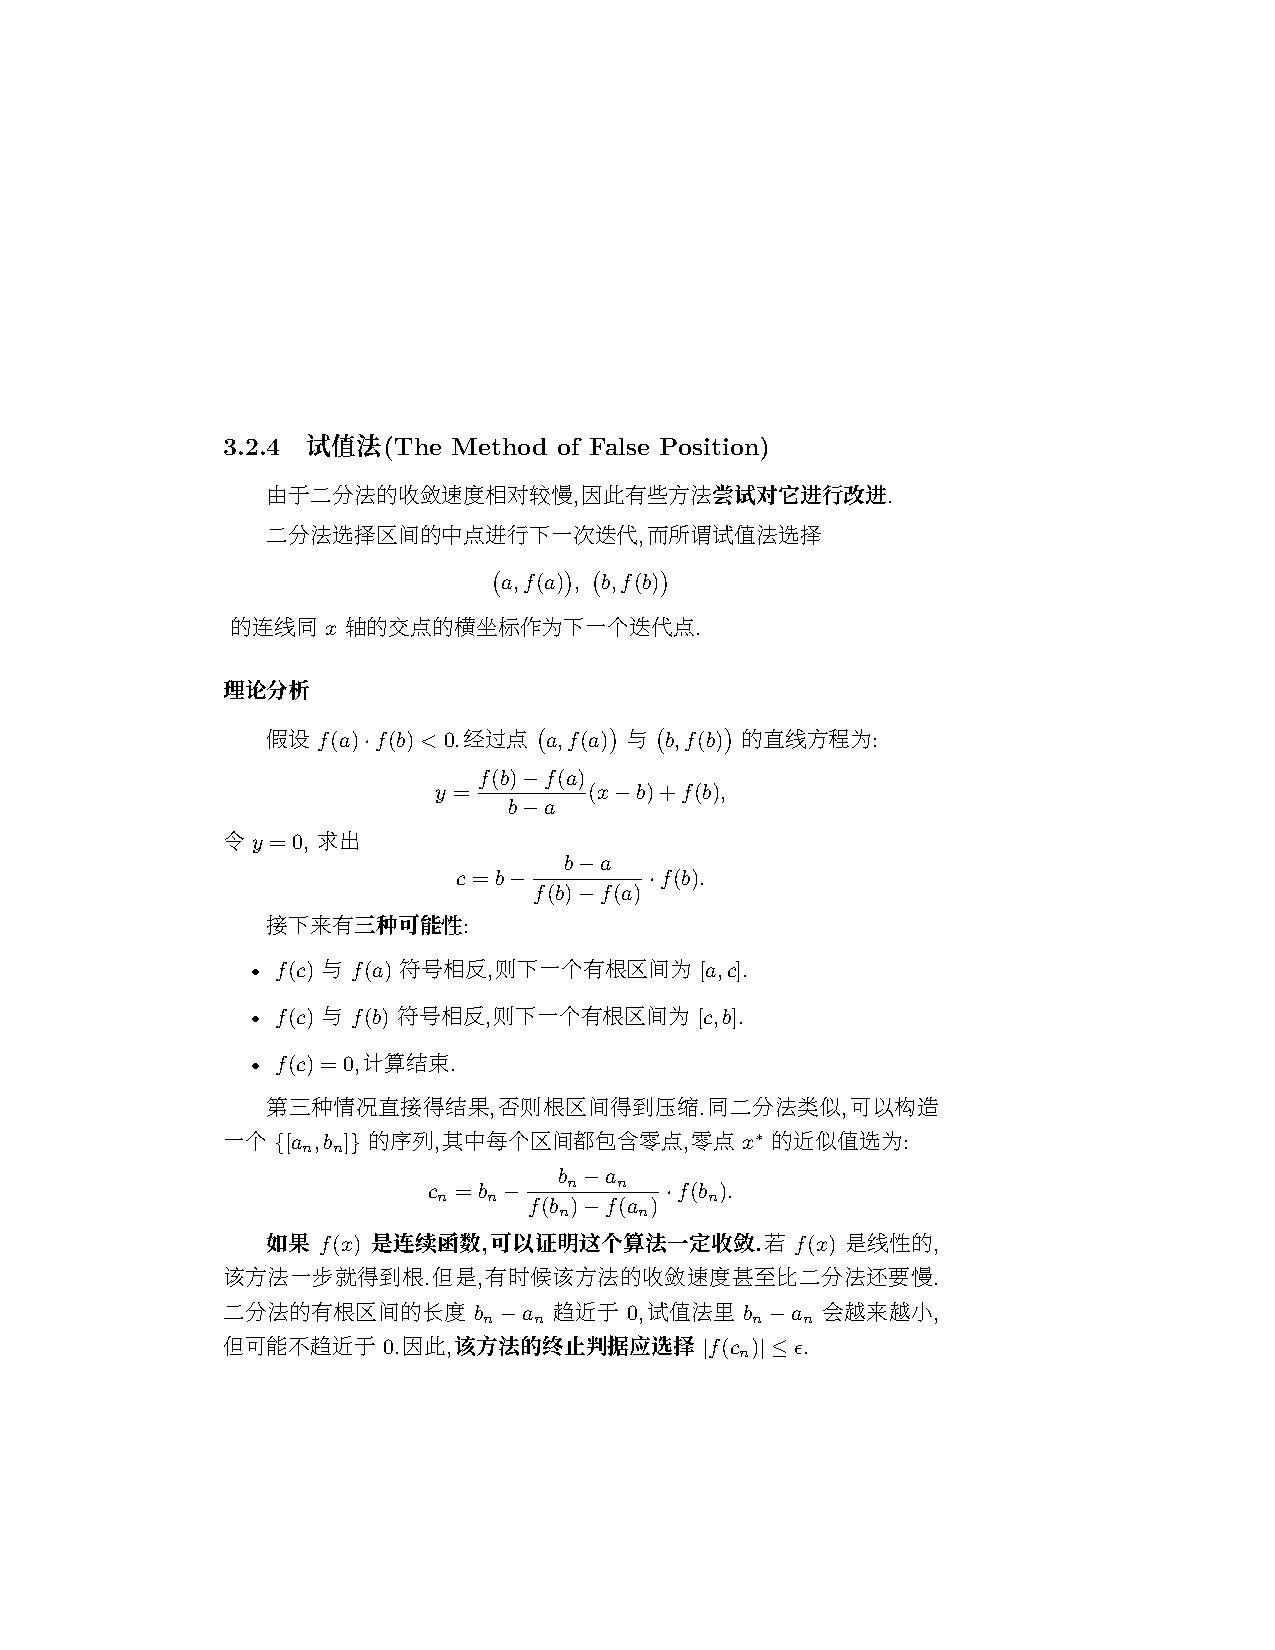
\includegraphics[width=\textwidth]{TVM}
  % \caption{试值法算法}
  % \label{fig:TVM}
\end{figure}

% subsection 问题1 (end)

\subsection{问题2} % (fold)
\label{sub:问题2}

\begin{figure}[ht]
\centering
  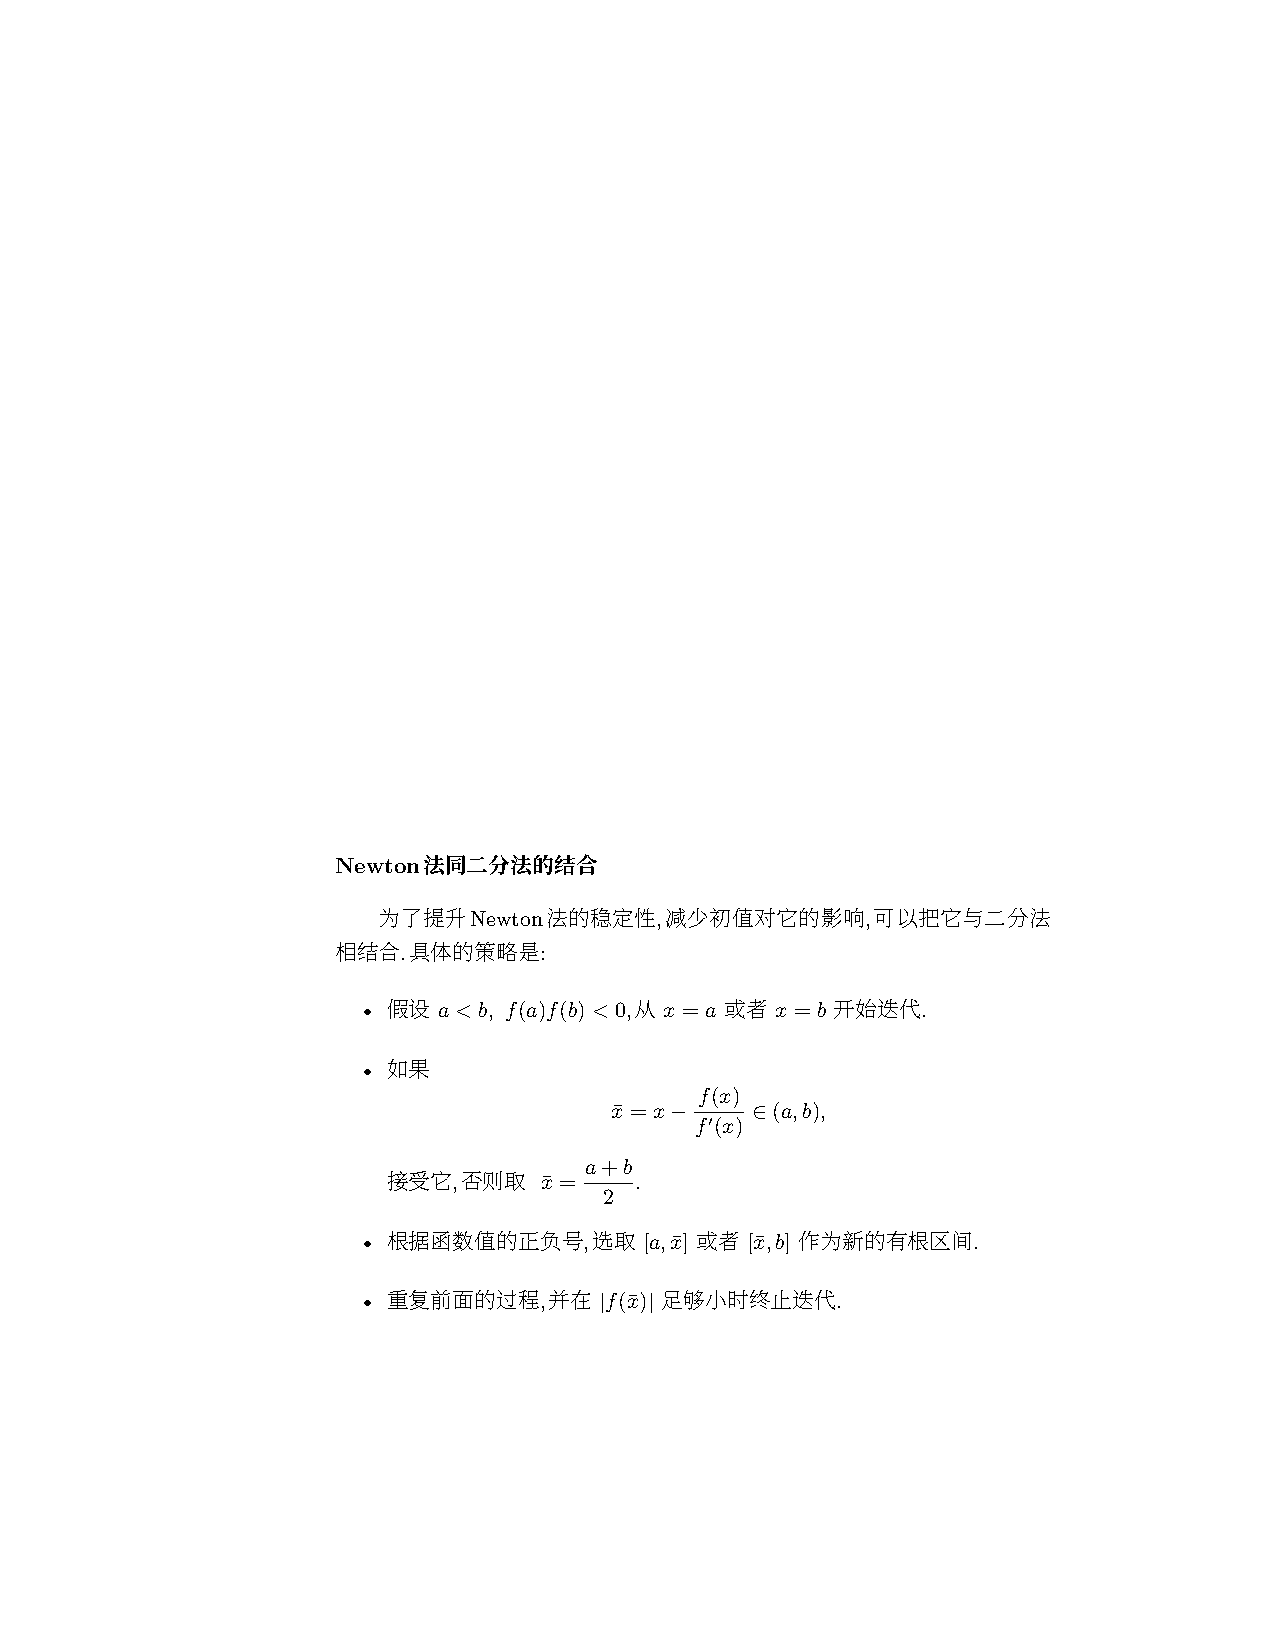
\includegraphics[width=\textwidth]{Newton}
  % \caption{Newton法同二分法结合}
  % \label{fig:Newton}
\end{figure}

% subsection 问题2 (end)


\section{分析}

\subsection{试值法流程}

图\ref{fig:TrailValueFlow} 为试值法算法流程图。

\begin{figure}[ht]
\centering
  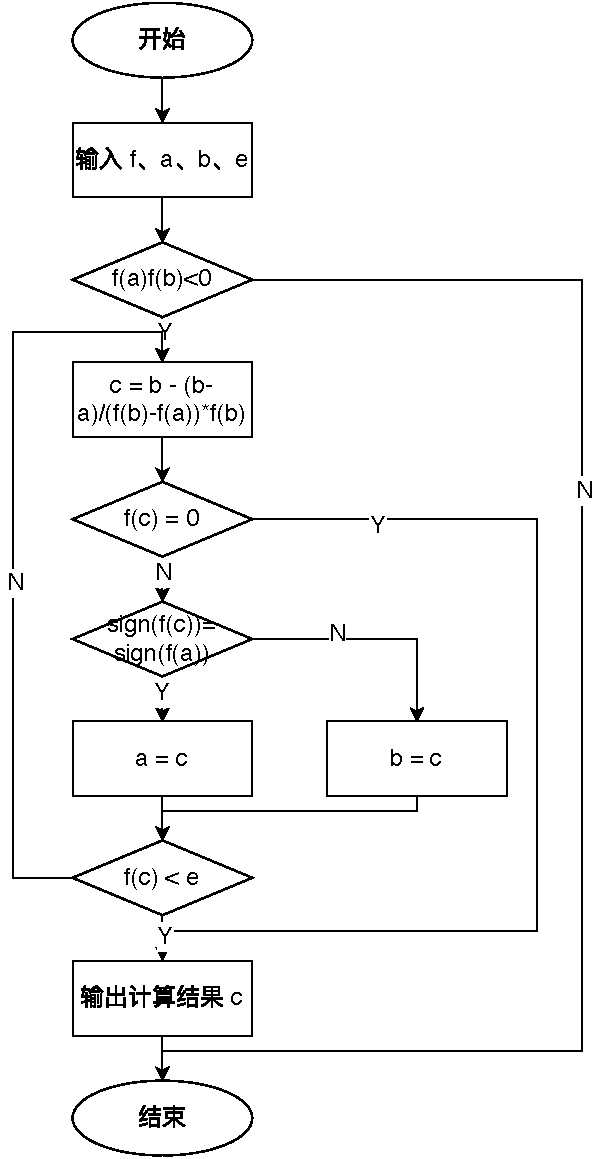
\includegraphics[width=0.5\textwidth]{TrailValueFlow}
  \caption{试值法流程图}
  \label{fig:TrailValueFlow}
\end{figure}

\subsection{Newton法同二分法结合流程}

图\ref{fig:NewtonFlow} 为试值法算法流程图。

\begin{figure}[ht]
\centering
  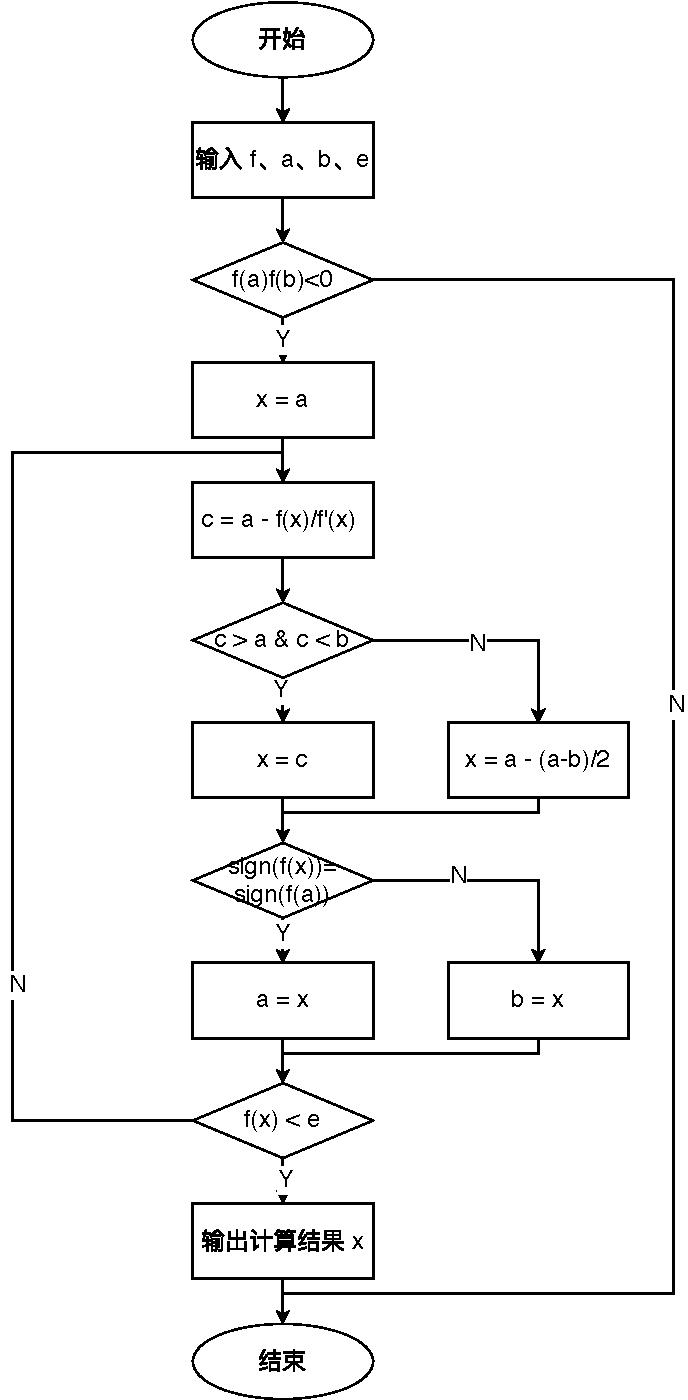
\includegraphics[width=0.5\textwidth]{Newton2Flow}
  \caption{Newton法同二分法结合流程}
  \label{fig:NewtonFlow}
\end{figure}

\section{程序}

试值法

\begin{lstlisting}[style = python]
def TrailValue(expr, a, b, e):
    """
    试值法
    f@函数
    a@区间下限
    b@区间上限
    e@容忍误差限
    """
    f = _func(expr)
    fa_0 = f.value(a)
    fb_0 = f.value(b)
    res = 0
    count = 0
    if abs(fa_0) < e:
        res = a
    elif abs(fb_0) < e:
        res = b
    elif sympy.sign(fa_0) == sympy.sign(fb_0):
        print('f(a) and f(b) 同号')
        sys.exit()
    else:
        while True:
            count = count + 1
            fa = f.value(a)
            fb = f.value(b)
            c = b - ((b-a)/(fb - fa))*fb
            fc = f.value(c)

            # 更新有根区间
            if sympy.sign(fa) == sympy.sign(fc):
                a = c
            else:
                b = c

            # 判断计算结束
            if abs(f.value(c)) < e:
                res = c
                break

    return res, count
\end{lstlisting}

Newton法同二分法结合

\begin{lstlisting}[style = python]
def Newton(expr, a, b, e):
    """
    牛顿法与二分法结合
    f@函数
    a@区间下限
    b@区间上限
    e@容忍误差限
    """
    f = _func(expr)
    fa_0 = f.value(a)
    fb_0 = f.value(b)
    res = 0
    count = 0
    if abs(fa_0) < e:
        res = a
    elif abs(fb_0) < e:
        res = b
    elif sympy.sign(fa_0) == sympy.sign(fb_0):
        print('f(a) and f(b) 同号')
        sys.exit()
    else:
        x = a
        while True:
            count = count + 1
            c = x - f.value(x)/f.diff_value(x)

            # Newton与二分法结合,找下一个点
            if (c > a) and (c < b):
                x = c
            else:
                x = a+(b-a)/2

            # 更新有根区间
            if sympy.sign(f.value(a)) == sympy.sign(f.value(x)):
                a = x
            else:
                b = x

            # 判断计算结束
            if abs(f.value(x)) < e:
                res = x
                break

    return res, count
\end{lstlisting}

\section{算例}

\begin{enumerate}
  \item $x\times sin(x) - 1 = 0$,有根区间为(1, 2),误差限为$1\times 10^{-5}$。

  \begin{lstlisting}[style = python]
  试值法 根: 1.11416, 迭代次数: 3
  牛顿法 根: 1.11416, 迭代次数: 2
  \end{lstlisting}
  
  \item $x^2 - 5 = 0$,有根区间为(2, 3),误差限为$1\times 10^{-5}$。

  \begin{lstlisting}[style = python]
  试值法 根: 2.23607, 迭代次数: 7
  牛顿法 根: 2.23607, 迭代次数: 3
  \end{lstlisting}

  \item $x^3 -3x + 2 = 0$,有根区间为(-2.5, -1.5),误差限为$1\times 10^{-5}$。

  \begin{lstlisting}[style = python]
  试值法 根: -2.00000, 迭代次数: 11
  牛顿法 根: -2.00000, 迭代次数: 4
  \end{lstlisting}

\end{enumerate}

\section{结论}

\begin{enumerate}
  \item 相比于试值法,Newton与二分法结合的算法收敛速度更快;

  \item Newton与二分法结合提升了原始Newton法的稳定性;

  \item 无论是试值法还是Newton与二分法结合的算法,都只能求解函数穿过x轴的根,不能求解函数与x轴相切的根,例如在算例3中,无法求解 $x = 1.0$ 的根。

  \begin{figure}[ht]
  \centering
    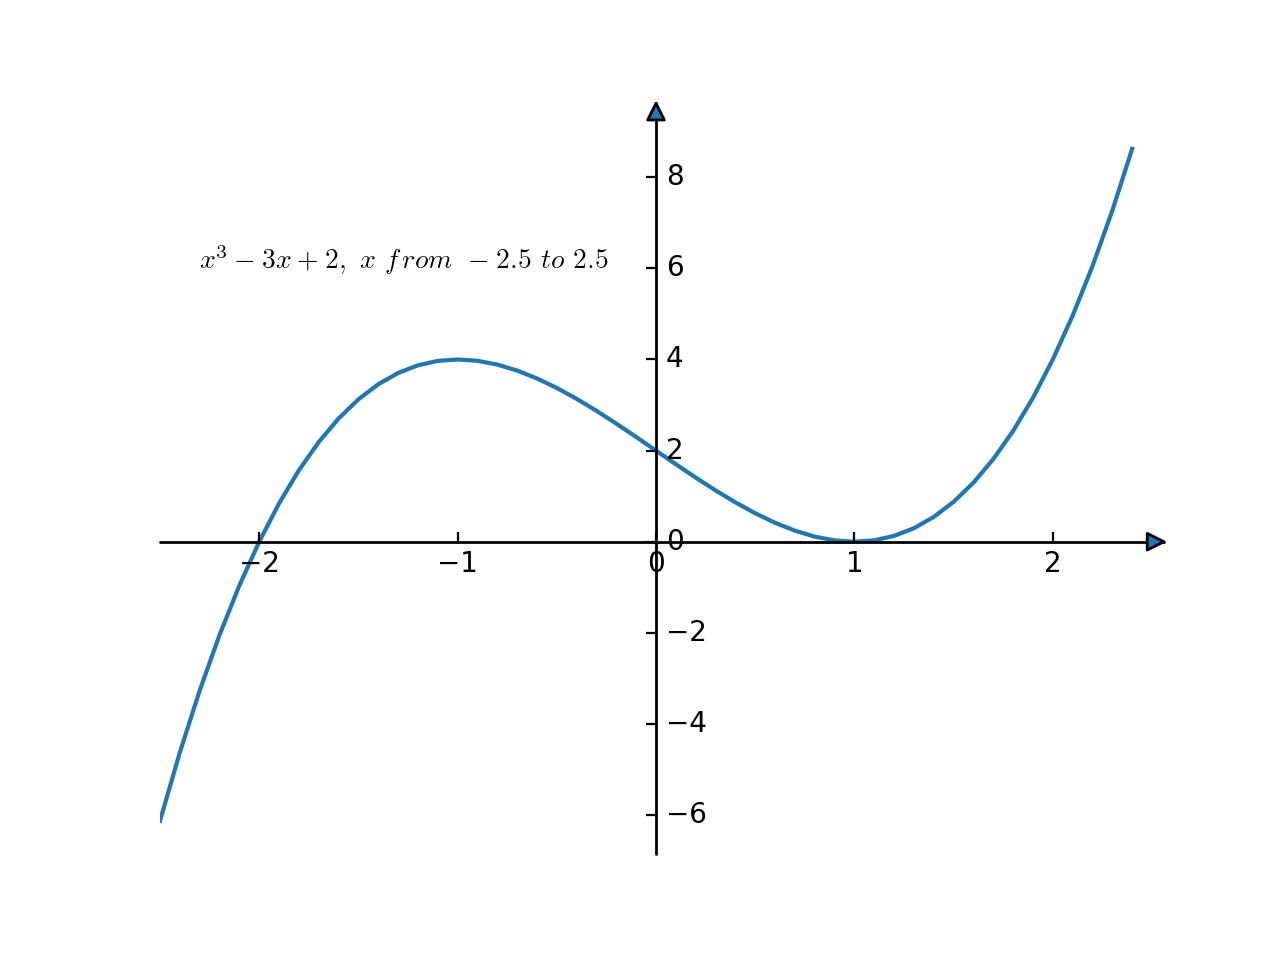
\includegraphics[width=0.6\textwidth]{f3}
    \caption{$f(x) = x^3 -3x + 2$}
    \label{fig:f3}
  \end{figure}

\end{enumerate}

% chapter chapter2 (end)